\documentclass[a4paper,11pt]{article}

% Kodovani (cestiny) v dokumentu: utf-8
%\usepackage[cp1250]{inputenc}	% Omezena stredoevropska kodova stranka, pouze MSW.
\usepackage[utf8]{inputenc}	% Doporucujeme pouzivat UTF-8 (unicode).

\usepackage[margin=2cm]{geometry}
\newtoks\jmenopraktika \newtoks\jmeno \newtoks\datum
\newtoks\obor \newtoks\skupina \newtoks\rocnik \newtoks\semestr
\newtoks\cisloulohy \newtoks\jmenoulohy
\newtoks\tlak \newtoks\teplota \newtoks\vlhkost

\jmenopraktika={Fyzikální praktikum 1}
\jmeno={Lukáš Lejdar}
\datum={15. října 2024}
\obor={F}
\skupina={Út 16:00}

\cisloulohy={9}
\jmenoulohy={Závislost indexu lomu skla na vlnové délce}

\tlak={101{,}35}
\teplota={21,1}
\vlhkost={47,7}


%%%%%%%%%%% Uzitecne balicky:
\usepackage[czech]{babel}

\usepackage{graphicx}
\usepackage{amsmath}
\usepackage{xspace}
\usepackage{url}
\usepackage{indentfirst}
\usepackage{wrapfig}
\usepackage{xcolor}
\usepackage{subfig}
\usepackage{subcaption}
\usepackage{enumitem}
\usepackage{tikzsymbols}
\usepackage{newfloat}

\DeclareFloatingEnvironment[fileext=lof]{graph}
\captionsetup[graph]{labelformat=simple, labelsep=colon, name=Graf}

%%%%%% Zamezeni parchantu:
\widowpenalty 10000 \clubpenalty 10000 \displaywidowpenalty 10000
%%%%%% Parametry pro moznost vsazeni vetsiho poctu obrazku na stranku
\setcounter{topnumber}{3}	  % max. pocet floatu nahore (specifikace t)
\setcounter{bottomnumber}{3}	  % max. pocet floatu dole (specifikace b)
\setcounter{totalnumber}{6}	  % max. pocet floatu na strance celkem
\renewcommand\topfraction{0.9}	  % max podil stranky pro floaty nahore
\renewcommand\bottomfraction{0.9} % max podil stranky pro floaty dole
\renewcommand\textfraction{0.1}	  % min podil stranky, ktery musi obsahovat text
\intextsep=8mm \textfloatsep=8mm  %\intextsep pro ulozeni [h] floatu a \textfloatsep pro [b] or [t]

% Tecky za cisly sekci:
\renewcommand{\thesection}{\arabic{section}.}
\renewcommand{\thesubsection}{\thesection\arabic{subsection}.}
% Jednopismenna mezera mezi cislem a nazvem kapitoly:
\makeatletter \def\@seccntformat#1{\csname the#1\endcsname\hspace{1ex}} \makeatother
%
\newcommand{\vsn}[4]{\ensuremath{#1 =} #2(#3)\,#4}
\newcommand{\vrn}[6]{\ensuremath{#1 =} (#2 $\pm$ #3)\,#4 ($p=$ #5\,\%, $\nu=$ #6)}

\newcommand*\circled[1]{\tikz[baseline=(char.base)]{
		\node[shape=circle,draw,inner sep=1pt] (char) {#1};}}

%%%%%%%%%%%%%%%%%%%%%%%%%%%%%%%%%%%%%%%%%%%%%%%%%%%%%%%%%%%%%%%%%%%%%%%%%%%%%%%
% Zacatek dokumentu
%%%%%%%%%%%%%%%%%%%%%%%%%%%%%%%%%%%%%%%%%%%%%%%%%%%%%%%%%%%%%%%%%%%%%%%%%%%%%%%

\begin{document}

\thispagestyle{empty}

{
\begin{center}
\sf 
{\Large Ústav fyziky a technologií plazmatu Přírodovědecké fakulty Masarykovy univerzity} \\
\bigskip
{\huge \bfseries FYZIKÁLNÍ PRAKTIKUM} \\
\bigskip
{\Large \the\jmenopraktika}
\end{center}

\bigskip

\sf
\noindent
\setlength{\arrayrulewidth}{1pt}
\begin{tabular*}{\textwidth}{@{\extracolsep{\fill}} l l}
\large {\bfseries Zpracoval:}  \the\jmeno & \large  {\bfseries Naměřeno:} \the\datum\\[2mm]
\large  {\bfseries Obor:} \the\obor  \hspace{40mm}  {\bfseries Skupina:} \the\skupina %
&\large {\bfseries Testováno:}\\
\\
\hline
\end{tabular*}
}

\bigskip

{
\sf
\noindent \begin{tabular}{p{4cm} p{0.6\textwidth}}
\Large  Úloha č. {\bfseries \the\cisloulohy:} \par
\smallskip
$T=\the\teplota$~$^\circ$C \par
$p=\the\tlak$~kPa \par
$\varphi=\the\vlhkost$~\%
&\Large \bfseries \the\jmenoulohy  \\[2mm]
\end{tabular}
}

\vskip1cm

\section{Úvod}

V úloze budu měřit index lomu hranolu metodou minimální deviace pro několik spektrálních čar rtuti. Z naměřených hodnot určím materiálové konstanty v Cauchyho vztahu a Abbeovo číslo charakterizovaného skla.
 
\section{Postup měření}

\subsection{Měření lámavého úhlu}

Dvě sousední strany hranolu, kterými paprsek vstupuje a vystupuje svírají úhel $ \omega $. Hranol položím na goniometr, který nejprve seřídím tak, aby stěny hranolu byli kolmé na optickou osu dalekohledu a najdu úhly $ \varphi_1 $ a $ \varphi_2 $, kdy je nitkový kříž kolmý na některou z těchto ploch. Vrcholový úhel dopočítám podle

\begin{equation}
\omega = 180 - (\varphi_1 - \varphi_2) 
\end{equation}

\subsection{Měření minimální deviace}

Paprsek se při průchodu takovým hranolem zlomí, o nějak úhel $ \delta $. Ze Snellova zákona lze zjistit, že existuje minimum této deviace $ \delta_m $, pro kterou platí

\begin{equation}
    n = \frac{\sin ((\delta_m + \omega) / 2)}{\sin (\omega / 2)}
\end{equation}

Zdrojem světla bude výbojka, která ve viditelné oblasti spektra obsahuje řadu čar o známých vlnových délkách. Budu otáčet se stolkem goniometru a hledat úhel $ \varphi_1 $, pro který deviace vykazuje minimum. Tuto hodnotu odečtu a budu se stolkem točit na druhou stranu dokud nenajdu druhé minimum $ \varphi_2 $. Úhel minimální deviace potom spočítám podle

\begin{equation}
2 \delta_m = \varphi_2 - \varphi_1
\end{equation}

Toto provedu pro každou spektrální čáru a dopočítám index lomu, který nutně bude různý pro různé vlnové délky. 

\begin{figure}
    \hfill
    \begin{minipage}[b]{.45\linewidth}
        \centering
        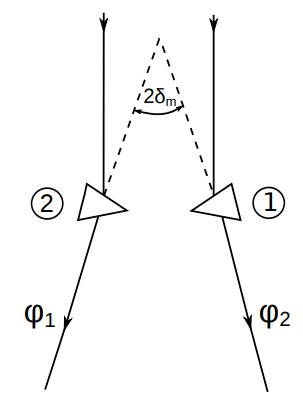
\includegraphics[width=0.4\textwidth]{mereni_minimalni_deviace.jpg}
        \caption{Měření úhlu minimální deviace}
    \end{minipage} 
    \hfill
    \begin{minipage}[b]{.45\linewidth}
        \centering
        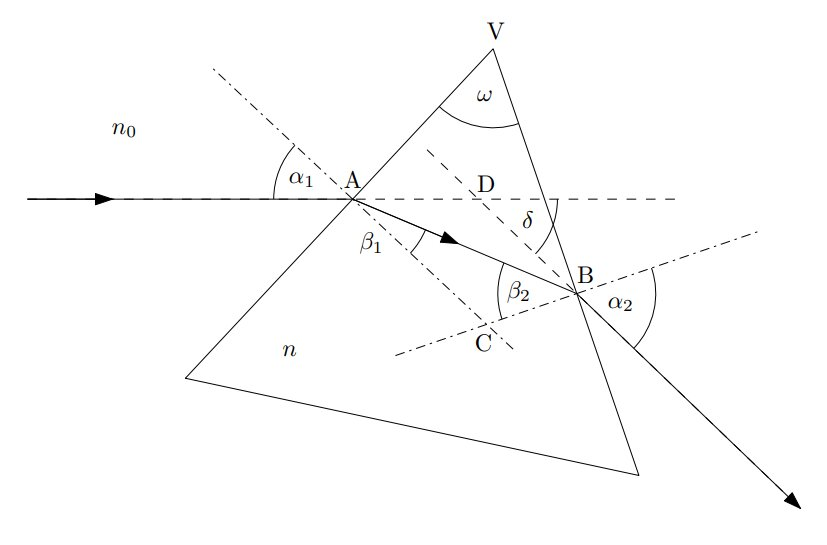
\includegraphics[width=\textwidth]{pruchod.jpg}
        \caption{Průchod paprsku světla hranolem}
    \end{minipage} 
    \hfill
\end{figure}

\subsection{Měření materiálových konstant Cauchyho vztahu a abbeova čísla}

Získanou závislost indexu lomu na vlnové délce budu prokládat Cauchyový vztahem prvního řádu

\begin{equation}
n = A + \frac{B}{\lambda^2}.
\end{equation}

Dvěma hlavními optickými parametry jsou index lomu $ n_d $ pro žlutou čáru $ \lambda_d = 587.6 $ nm a Abbeovo číslo $ \nu_d $, které je převrácenou hodnotou optické mohutnosti skla

\begin{equation}
\nu_d = \frac{n_d - 1}{n_F - n_C},
\end{equation}

\noindent
kde  $ n_F $ a $ n_C $ jsou indexy lomu pro Fraunhoferovy čáry o vlnových déklách $ \lambda_F = 486.1 $ nm (modrá) a $ \lambda_C = 656.3 $ nm (červená).

\newpage
\section{Výsledky měření}

\subsection{Měření lámavého úhlu}

Hranol umístím na goniometr a provedu justování. Srovnám nitkový kříž se stranami hranolu, svírajícími úhel $ \omega $ a odečtu úhly $ \varphi_1 $ a $ \varphi_2 $. Vrcholový úhel dopočítám podle (1).

\begin{equation}
\omega = 45.00^{\circ} \pm 0.05
\end{equation}

\subsection{Měření minimální deviace}

Měření úhlu minimální deviace $ \delta_m $ provádím pro každou spektrální čáru rtuti v bodě obratu paprsku na obou stranách, při otáčení stolečkem goniometru a index lomu dopočítávám podle (2).

\begin{table}[htpb]
    \centering
    \begin{tabular}{lccc}
        \hline\hline
        barva & $ \lambda $ (nm) & $ \delta_m $ $ (^{\circ}) $ & n \\\hline
        červená & 623.4 &  30.8402 & $1.6059 \pm 0.0008$ & 
        žlutá & 576.9 &  30.9638 & $1.6082 \pm 0.0008$ & 
        zelená & 546.1 &  31.0513 & $1.6097 \pm 0.0008$ & 
        modro-zelená & 491.6 &  31.3444 & $1.6150 \pm 0.0008$ & 
        modrá & 435.8 &  31.7132 & $1.6216 \pm 0.0008$ & 
        fialová & 404.6 &  31.9069 & $1.6250 \pm 0.0008$ & 
        \hline\hline
    \end{tabular}
    \caption{Měření úhlu minimální deviace pro každou spektrální čáru rtuti}
\end{table}

\subsection{Měření materiálových konstant Cauchyho vztahu a abbeova čísla}

Vynesl jsem do grafu závislost indexu lomu $ n $ na vlnové délce $ \lambda $ a hodnoty proložil Cauchyovým vztahem (4). Uvedl jsem výsledné materiálové konstanty $ A $ a $ B $ a vzorkoval jsem výslednou funkci v Fraunhoferových vlnových délkách pro výpočet Abbeova čísla $ \nu_d $.

\begin{align*}
    n_d &= 1.608 \pm 0.001 && A = 1.5915 \pm 0.0008  \\
    n_F &= 1.615 \pm 0.001 && B = 5.6 \pm 0.2 \cdot 10^{-15} \text{ m}^2 \\
    n_C &= 1.604 \pm 0.0009 \\
    \nu_d &= 57 \pm 2
\end{align*}

\begin{figure}[htpb]
    \centering
    % GNUPLOT: LaTeX picture with Postscript
\begingroup
  \makeatletter
  \providecommand\color[2][]{%
    \GenericError{(gnuplot) \space\space\space\@spaces}{%
      Package color not loaded in conjunction with
      terminal option `colourtext'%
    }{See the gnuplot documentation for explanation.%
    }{Either use 'blacktext' in gnuplot or load the package
      color.sty in LaTeX.}%
    \renewcommand\color[2][]{}%
  }%
  \providecommand\includegraphics[2][]{%
    \GenericError{(gnuplot) \space\space\space\@spaces}{%
      Package graphicx or graphics not loaded%
    }{See the gnuplot documentation for explanation.%
    }{The gnuplot epslatex terminal needs graphicx.sty or graphics.sty.}%
    \renewcommand\includegraphics[2][]{}%
  }%
  \providecommand\rotatebox[2]{#2}%
  \@ifundefined{ifGPcolor}{%
    \newif\ifGPcolor
    \GPcolorfalse
  }{}%
  \@ifundefined{ifGPblacktext}{%
    \newif\ifGPblacktext
    \GPblacktexttrue
  }{}%
  % define a \g@addto@macro without @ in the name:
  \let\gplgaddtomacro\g@addto@macro
  % define empty templates for all commands taking text:
  \gdef\gplbacktext{}%
  \gdef\gplfronttext{}%
  \makeatother
  \ifGPblacktext
    % no textcolor at all
    \def\colorrgb#1{}%
    \def\colorgray#1{}%
  \else
    % gray or color?
    \ifGPcolor
      \def\colorrgb#1{\color[rgb]{#1}}%
      \def\colorgray#1{\color[gray]{#1}}%
      \expandafter\def\csname LTw\endcsname{\color{white}}%
      \expandafter\def\csname LTb\endcsname{\color{black}}%
      \expandafter\def\csname LTa\endcsname{\color{black}}%
      \expandafter\def\csname LT0\endcsname{\color[rgb]{1,0,0}}%
      \expandafter\def\csname LT1\endcsname{\color[rgb]{0,1,0}}%
      \expandafter\def\csname LT2\endcsname{\color[rgb]{0,0,1}}%
      \expandafter\def\csname LT3\endcsname{\color[rgb]{1,0,1}}%
      \expandafter\def\csname LT4\endcsname{\color[rgb]{0,1,1}}%
      \expandafter\def\csname LT5\endcsname{\color[rgb]{1,1,0}}%
      \expandafter\def\csname LT6\endcsname{\color[rgb]{0,0,0}}%
      \expandafter\def\csname LT7\endcsname{\color[rgb]{1,0.3,0}}%
      \expandafter\def\csname LT8\endcsname{\color[rgb]{0.5,0.5,0.5}}%
    \else
      % gray
      \def\colorrgb#1{\color{black}}%
      \def\colorgray#1{\color[gray]{#1}}%
      \expandafter\def\csname LTw\endcsname{\color{white}}%
      \expandafter\def\csname LTb\endcsname{\color{black}}%
      \expandafter\def\csname LTa\endcsname{\color{black}}%
      \expandafter\def\csname LT0\endcsname{\color{black}}%
      \expandafter\def\csname LT1\endcsname{\color{black}}%
      \expandafter\def\csname LT2\endcsname{\color{black}}%
      \expandafter\def\csname LT3\endcsname{\color{black}}%
      \expandafter\def\csname LT4\endcsname{\color{black}}%
      \expandafter\def\csname LT5\endcsname{\color{black}}%
      \expandafter\def\csname LT6\endcsname{\color{black}}%
      \expandafter\def\csname LT7\endcsname{\color{black}}%
      \expandafter\def\csname LT8\endcsname{\color{black}}%
    \fi
  \fi
    \setlength{\unitlength}{0.0500bp}%
    \ifx\gptboxheight\undefined%
      \newlength{\gptboxheight}%
      \newlength{\gptboxwidth}%
      \newsavebox{\gptboxtext}%
    \fi%
    \setlength{\fboxrule}{0.5pt}%
    \setlength{\fboxsep}{1pt}%
    \definecolor{tbcol}{rgb}{1,1,1}%
\begin{picture}(5760.00,2880.00)%
    \gplgaddtomacro\gplbacktext{%
      \csname LTb\endcsname%%
      \put(1078,372){\makebox(0,0)[r]{\strut{}$1.605$}}%
      \put(1078,848){\makebox(0,0)[r]{\strut{}$1.61$}}%
      \put(1078,1325){\makebox(0,0)[r]{\strut{}$1.615$}}%
      \put(1078,1801){\makebox(0,0)[r]{\strut{}$1.62$}}%
      \put(1078,2278){\makebox(0,0)[r]{\strut{}$1.625$}}%
      \put(1518,-134){\makebox(0,0){\strut{}$400$}}%
      \put(2287,-134){\makebox(0,0){\strut{}$450$}}%
      \put(3056,-134){\makebox(0,0){\strut{}$500$}}%
      \put(3825,-134){\makebox(0,0){\strut{}$550$}}%
      \put(4594,-134){\makebox(0,0){\strut{}$600$}}%
      \put(5363,-134){\makebox(0,0){\strut{}$650$}}%
    }%
    \gplgaddtomacro\gplfronttext{%
      \csname LTb\endcsname%%
      \put(4376,2486){\makebox(0,0)[r]{\strut{}fit}}%
      \csname LTb\endcsname%%
      \put(209,1372){\rotatebox{-270.00}{\makebox(0,0){\strut{}$n$}}}%
      \put(3286,-464){\makebox(0,0){\strut{}$\lambda$ (nm)}}%
    }%
    \gplbacktext
    \put(0,0){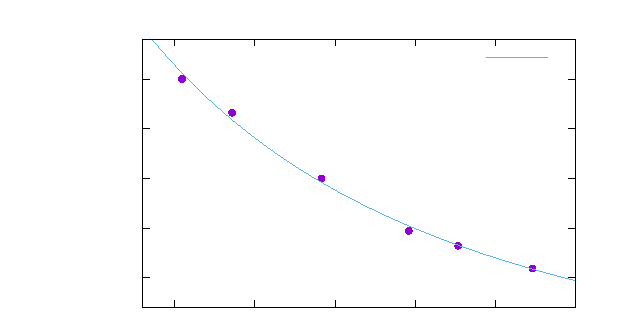
\includegraphics[width={288.00bp},height={144.00bp}]{cauchy}}%
    \gplfronttext
  \end{picture}%
\endgroup

    \captionsetup{type=graph}
    \caption{Závislost indexu lomu na vlnové délce}
\end{figure}

\section{Závěr}

Změřil jsem lámavý úhel hranolu a minimální deviaci pro několik spektrálních čar rtuti. Výsledné hodnoty, které jsou uvedeny v tabulce 1 jsem dál fitoval Cauchyovým vztahem a dostal materiálové konstanty A a B, a zjistil index lomu pro žlutou čáru $ n_d = 1.608 \pm 0.001 $ a Abbeovo číslo $ \nu_d = 57 \pm 2 $. 

Použitý hranol byl z materiálu $ N-SK2 $ výrobce SCHOTT. Tabulkové hodnoty z odkazu 1 jsou $ n_d = 1.60738 $ a $ \nu_d = 56.65 $.

\begin{thebibliography}{0}
\bibitem{N-SK2} tabulkové hodnoty hranolů N-SK2 SCHOTT~\url{https://www.schott.com/shop/advanced-optics/en/Optical-Glass/N-SK2/c/glass-N-SK2}.   
\end{thebibliography}

\end{document}
